\section{TransFuser}
\label{sec:transfuser}

%  deep dive i transfuser (hvordan den fungerer, hvordan man gjør modifikasjoner)
% få med challenges on multi-modal sensors


\begin{comment}
    Hva er egentlig viktig å ha med her? En forkortet versjon av paperet? Skal vi heller ta utgangspunkt i hvordan koden deres er satt opp?

Fra paperet:
3 Transfuser
3.1 Problem setting -- basically IL, dette har vi beskrevet
3.2 Input and Output Paramtererization
3.3 Multi-Modal Fusion Transformer -- denne er viktig?
3.4 Waypoint Prediction Network
3.5 Controller   <---
3.6 Loss Functions

4 Experiments
4.1 Task
4.2 Training dataset hello\textsuperscript{hello\textsuperscript{hello}} is there anybody in there just nod if you can hear me is there anyone at home
4.3 Expert
4.4 Longest6 Benchmark --- dette har vi beskrevet
4.5 Metrics --- dette har vi beskrevet
4.6 Baselines -- urelevant?
4.7 Implementation details
...
\end{comment}


This specialization project experiments with the work proposed by \textcite{transfuser-pami}. This section will therefore describe the TransFuser model in more detail, and is heavily based on their paper. They consider a  Behavior Cloning approach where the goal is safe point-to-point navigation in an urban setting. 

\subsection{Training Data}
An expert policy is first rolled out in the environment to collect a high-dimensional dataset which consists of observations of the environment and corresponding expert trajectory. Each time step in the dataset includes a front camera image input and LIDAR point cloud data, while the expert trajectory is defined by a set of 2D waypoints in \acrfull{bev} space which uses the coordinate frame of the ego-vehicle. \textcite{transfuser-pami} use all of the 8 included towns in CARLA version 0.9.10 to generate data. The dataset is based on around 2500 routes through junctions with an average length of 100 meters, and 1000 routes along curved highways with an average length of 400 meters. This results in a dataset containing 228,000 frames in total.

The expert policy use information made available by the simulator to generate data at 2 FPS. The policy constructed using an A* planner followed by two PID controllers for lateral and longitudinal control. Lateral control is done by minimizing the angle of the car towards the next waypoint in the route. Longitudinal control is done using model predictive control. The standard target speed is 4.0 m/s. This is reduced to 3.0 m/s while the expert is in a intersection. Finally, a predicted infraction sets the target speed to 0.0 m/s. Collision infractions are predicted by forecasting the position of all traffic participants based on a pretrained kinematic bicycle model, while red light infractions are predicted by performing intersection tests with trigger boxes provided by CARLA.

\subsection{Model Architecture}
The TransFuser model has two main components. A multi-modal fusion transformer integrates information from RGB images and LIDAR data. This is then fed into an auto-regressive network for predicting waypoints that are used to control the autonomous vehicle. The following sub-sections will describe the components seen in \cref{fig:alt-transfuser-architecture}.

\begin{figure}
    \centering
    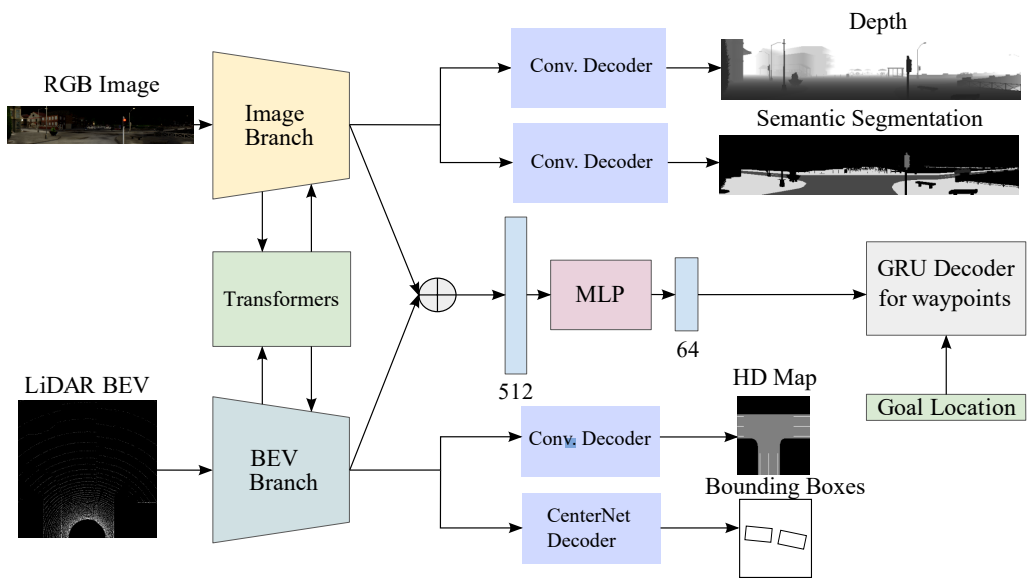
\includegraphics[width=\textwidth]{figures/3/transfuser.png}
    \caption{An overview of TransFuser architecture. Multi-modal Fusion Transformer creates two branches that are combined and fed into an MLP before passing it to an auto-regressive waypoint prediction network. The branches are also used for auxiliary tasks. Source: \cite{transfuser-pami}.}
    \label{fig:alt-transfuser-architecture}
\end{figure}

\subsubsection{Input}
The model receives data from two modalities as input. The first is a three-channel image of size 256$\times$256 pixels representing a 2D LIDAR BEV around the vehicle. The first two channels consist of a 2-bin histogram created from the raw LIDAR point cloud, where each bin represent the point on/below and above the ground plane. The last channel includes the 2D goal location converted into the same BEV space. The other modality comes from three front-facing RGB cameras with a 60$^\circ$ spacing. The three images are combined into a single image with resolution 704$\times$160 pixels and 132$^\circ$ field of view.

\subsubsection{Multi-Modal Fusion Transformer}
\textcite{transfuser-pami} use the self-attention mechanism of Transformers to incorporate global context from complementary RGB images and LIDAR data. Using self-attention in natural language processing tasks normally means working with token input and output structures, but when working with image data they instead work on grid structured feature maps. TransFuser performs dense feature fusion at multiple resolutions to obtain a feature map from both the RGB images and the BEV LIDAR data. They are then reduced to a dimension of 512 by average pooling and followed by a fully-connected layer at each branch. The output feature vectors from each modality is then combines via summation, which results in a compact representation of the environment that encodes the global context of the 3D scene. See \cref{sec:related-work:transfuser} for a detailed visualization of this component.

\subsubsection{Waypoint Prediction Network}
The 512-dimensional feature vector from the Multi-Modal Fusion Transformer is passed through a multilayer perceptron to reduce its dimensionality to 64 to increase computational efficiency. This output, in addition to the current position and goal location, is then fed into a waypoint prediction network implemented using gated recurrent units (GRUs). This results in waypoint predictions for four future time-steps in the ego-vehicle coordinate frame.

\subsubsection{Loss Functions and Auxiliary Tasks}
The primary loss function is based on the $L_1$ distance between the above predicted waypoints and the expert trajectory. Additionally, several auxiliary losses are used to increase interpretability and robustness in the model. 2D depth and semantic segmentation are decoded from the image branch features and are supervised with $L_1$ loss and cross-entropy loss respectively. A high definition BEV map classifying roads, lane markings and more is used to encourage the model to encode information regarding drivable and non-drivable areas. This is created from the LIDAR branch using a convolutional decoder and use cross-entropy loss. Finally, a position map containing bounding boxes for other vehicles is predicted from the LIDAR branch using a convolutional decoder.

\subsubsection{Output}
The final output of the model is the predicted future trajectory of the ego-vehicle in BEV space. This is represented by a sequence of four 2D waypoints.


\subsection{Controlling the Vehicle}
PID controllers use the predicted waypoints to perform low-level control of the vehicle, such as acceleration, steering and braking. TransFuser implements one controller each for the lateral and longitudinal direction. The model additionally implements two functions for more refined control. Creeping is used to wake up the vehicle if it has been stationary for a long duration, which is useful to counteract how vehicles tend to stand still in much of the training data due to dense traffic. Still, creeping would not be safe in a situation where the vehicle actually is stuck in traffic with another vehicle in front of it. Therefore a safety heuristic is implemented that disables the creeping behaviour based on LIDAR data in a small area in front of the car. 


\subsection{Upgrading TransFuser to CARLA Version 0.9.13}
% beskrive hva som måtte endred i kodebasen til TransFuser for å få den kompatibel med 0.9.13

TransFuser was originally designed for CARLA version 0.9.10.
The simulator has since then been improved and updated to version 0.9.13,
and we therefore wanted to modify TransFuser to work with this version.
The main motivation for the upgrade is the improved support for headless mode,
which is a requirement for running the simulator on the Idun HPC cluster.

To do this, we forked the project and made the necessary adjustments to be compatible with the new CARLA version's API.
No major structural changes where needed,
the API changes mainly consisted of classes and functions being renamed.
Specific details can be found in the git log on the branch named \texttt{0.9.13}.

% \todo[inline]{greit nok?} tyy

